\documentclass{ML}
\usepackage{float}
% 姓名,学号
\infoauthor{朱明彦}{1160300314}

% 课程类型,实验名称
\infoexp{课程类型}{实验一}

\infoschool{计算机学院}{高宏}

\begin{document}
\maketitle

% \tableofcontents
\newpage

\begin{center}
    \textbf{\zihao{3} 实验一 MySQL关系数据库管理系统及SQL语言的使用}
\end{center}

\section{实验目的}
    掌握 MySQL 关系数据库管理系统的基本命令,并熟练使用 SQL 语言管理
MySQL 数据库。掌握 SQL 语言的使用方法,学会使用 SQL 语言进行关系数据
库查询,特别是聚集查询、连接查询和嵌套查询。
\section{实验环境}
\begin{itemize}
    \item Ubuntu 16.04.5
    \item MySQL Ver 14.14 Distrib 5.7.25
\end{itemize}
\section{实验过程及结果}
% 对报告中第 3 部分的实验结果进行截图,作为评分标准。对于 3.2,使用
% MYSQL 基本命令可以查看创建的关系数据库的每个模式(参看第 4 部分 MYSQL
% 手册,做作业之前先练习第 4 部分有助于熟悉 MYSQL 命令),对结果进行截图。
% 对于 3.3,使用 select *语句分别显示每张表中被添加的数据,对结果进行截图。
% 对于 3.1,在你完成 3.2 和 3.3 之后,把输入的 9 条 sql 语句和相应的查询结果截
% 图显示,所以你设计的数据库必须包括 3.1 需要的各种数据。
\subsection{实验任务}
\begin{enumerate}
    \item 参加了项目名为"SQL Project"的员工的名字;
    \begin{minted}{SQL}
    SELECT ENAME
    FROM EMPLOYEE, WORKS_ON, PROJECT
    WHERE EMPLOYEE.ESSN = WORKS_ON.ESSN AND WORKS_ON.PNO = PROJECT.PNO
        AND PROJECT.PNAME = "SQL Project";
    \end{minted}
    SQL查询结果如图\ref{fig:1}
    \begin{figure}[htb]
        \centering
        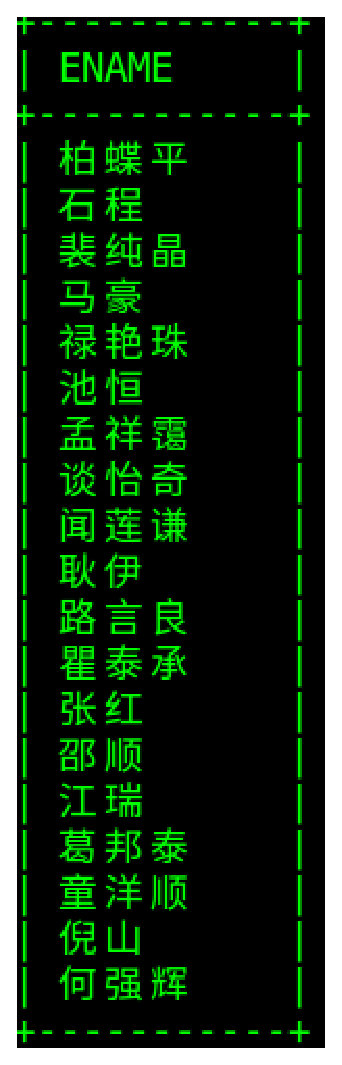
\includegraphics[scale=0.4, bb=0 0 148 495]{media/3.1.1.eps}
        \caption{}\label{fig:1}
    \end{figure}
    \item 在"Research Department"工作且工资低于3000元的员工名字和地址;
    \begin{minted}{SQL}
    SELECT ENAME, ADDRESS
    FROM EMPLOYEE, DEPARTMENT
    WHERE EMPLOYEE.DNO = DEPARTMENT.DNO 
        AND DEPARTMENT.DNAME = "Research Department"
        AND SALARY < 3000;
    \end{minted}
    SQL查询结果如图\ref{fig:2}
    \begin{figure}[htb]
        \centering
        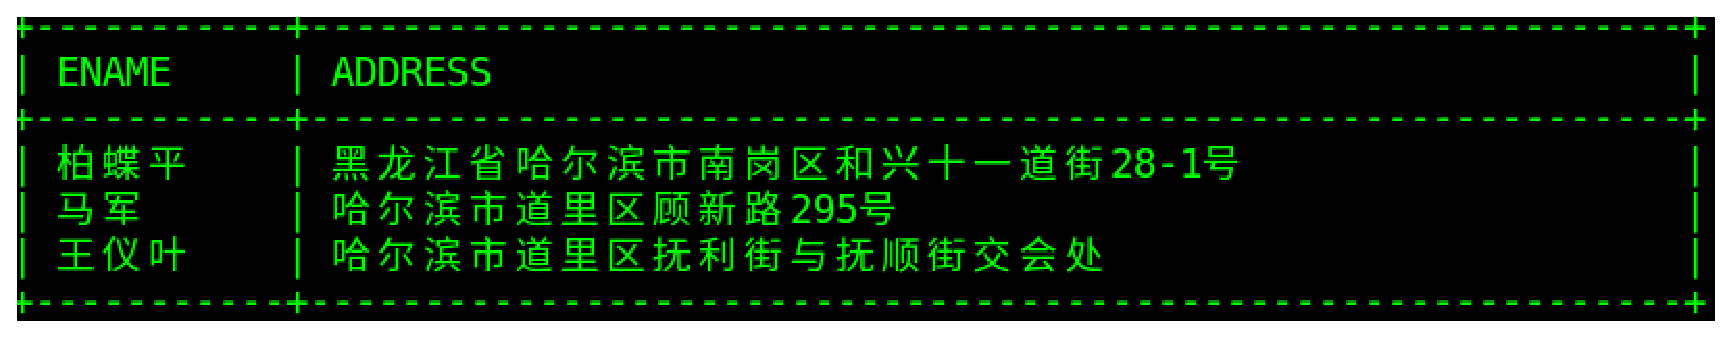
\includegraphics[scale=0.5, bb=0 0 815 146]{media/3.1.2.eps}
        \caption{}\label{fig:2}
    \end{figure}
    \item 没有参加项目编号为P1的项目的员工名字;
    \begin{minted}{SQL}
    SELECT DISTINCT ENAME
    FROM EMPLOYEE
    WHERE ENAME NOT IN(
        SELECT DISTINCT ENAME
        FROM EMPLOYEE, WORKS_ON
        WHERE WORKS_ON.ESSN = EMPLOYEE.ESSN AND WORKS_ON.PNO = "P1"
    );
    \end{minted}

    SQL查询结果如图\ref{fig:3},但由于总的查询结果有70条,故此处仅列出部分查询结果。
    \begin{figure}[htb]
        \centering
        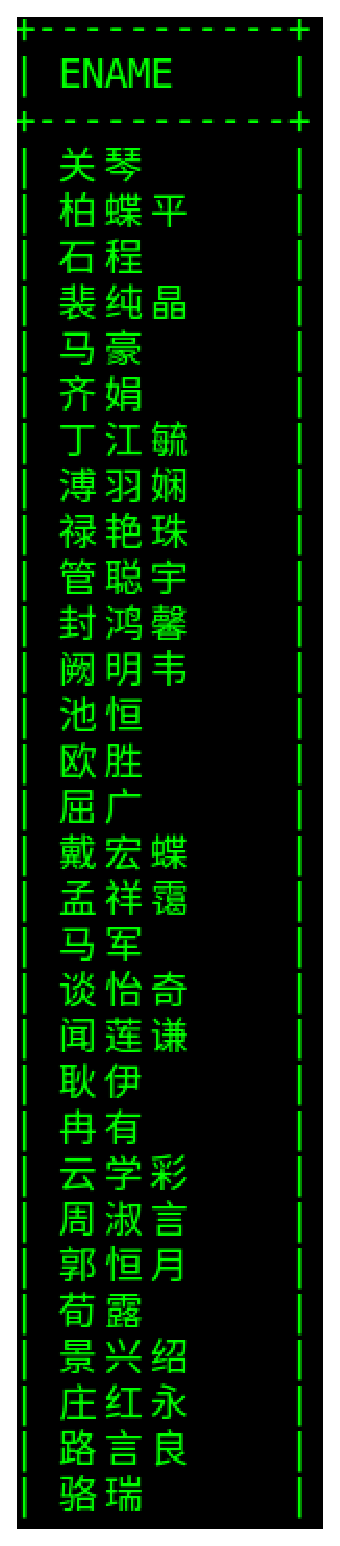
\includegraphics[scale=0.4, bb=0 0 147 726]{media/3.1.3.eps}
        \caption{}\label{fig:3}
    \end{figure}
    \item 由张红领导的工作人员的姓名和所在部门;
    \begin{minted}{SQL}
    SELECT ENAME, DNAME
    FROM DEPARTMENT, EMPLOYEE
    WHERE EMPLOYEE.DNO = DEPARTMENT.DNO 
        AND EMPLOYEE.SUPERSSN IN(
            SELECT ESSN
            FROM EMPLOYEE
            WHERE ENAME = "张红"
        );
    \end{minted}
    SQL查询结果如图\ref{fig:4}
    \begin{figure}[htb]
        \centering
        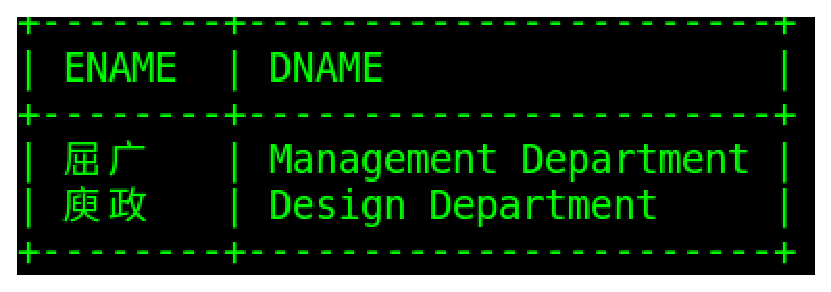
\includegraphics[scale=0.4, bb=0 0 383 124]{media/3.1.4.eps}
        \caption{}\label{fig:4}
    \end{figure}
    \item 至少参加了项目编号为P1和P2的项目的员工号;
    \begin{minted}{SQL}
    SELECT DISTINCT ESSN
    FROM WORKS_ON
    WHERE PNO = "P1" 
    AND ESSN IN(
        SELECT DISTINCT ESSN
        FROM WORKS_ON
        WHERE PNO = "P2"
    );
    \end{minted}
    SQL查询结果如图\ref{fig:5}
    \begin{figure}[htb]
        \centering
        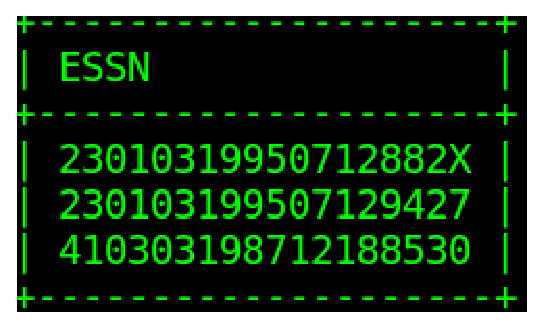
\includegraphics[scale=0.4, bb=0 0 245 142]{media/3.1.5.eps}
        \caption{}\label{fig:5}
    \end{figure}
    \item 参加了全部项目的员工号码和姓名;
    \begin{minted}{SQL}
    SELECT DISTINCT R1.ESSN, ENAME 
    FROM WORKS_ON R1, EMPLOYEE
    WHERE NOT EXISTS(
        SELECT PROJECT.PNO FROM PROJECT
        WHERE NOT EXISTS(
            SELECT * FROM WORKS_ON R2
            WHERE R2.ESSN = R1.ESSN AND R2.PNO = PROJECT.PNO
        )
    ) AND R1.ESSN = EMPLOYEE.ESSN;
    \end{minted}
    SQL查询结果如图\ref{fig:6}
    \begin{figure}[htb]
        \centering
        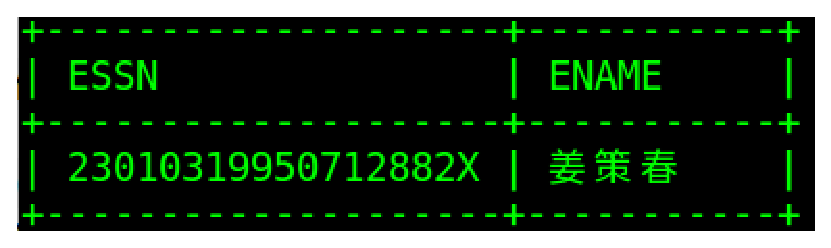
\includegraphics[scale=0.4, bb=0 0 383 103]{media/3.1.6.eps}
        \caption{}\label{fig:6}
    \end{figure}
    \item 员工平均工资低于3000元的部门名称;
    \begin{minted}{SQL}
    SELECT DNAME
    FROM DEPARTMENT, EMPLOYEE
    WHERE DEPARTMENT.DNO = EMPLOYEE.DNO
    GROUP BY DEPARTMENT.DNO
    HAVING AVG(SALARY) < 3000;
    \end{minted}
    SQL查询结果如图\ref{fig:7}
    \begin{figure}[htb]
        \centering
        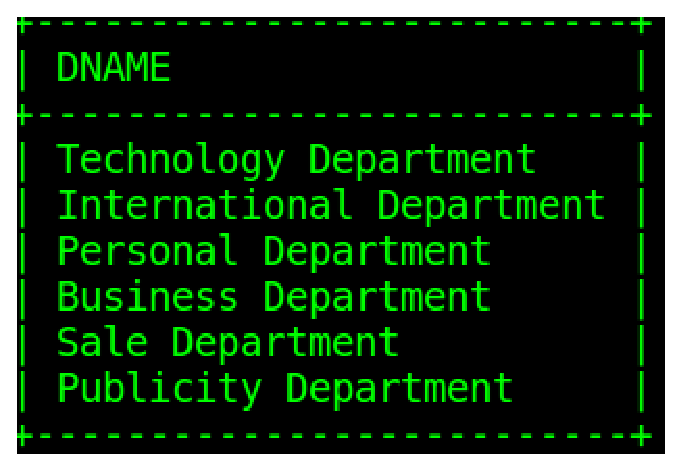
\includegraphics[scale=0.4, bb=0 0 311 210]{media/3.1.7.eps}
        \caption{}\label{fig:7}
    \end{figure}
    \item 至少参与了3个项目且工作总时间不超过8小时的员工名字;
    \begin{minted}{SQL}
    SELECT ENAME FROM EMPLOYEE
    WHERE ESSN IN(
        SELECT ESSN
        FROM WORKS_ON
        GROUP BY ESSN HAVING COUNT(PNO) >= 3 AND SUM(HOURS) <= 8
    );
    \end{minted}
    SQL查询结果如图\ref{fig:8}
    \begin{figure}[htb]
        \centering
        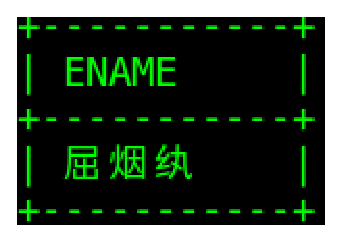
\includegraphics[scale=0.4, bb=0 0 148 100]{media/3.1.8.eps}
        \caption{}\label{fig:8}
    \end{figure}
    \item 每个部门员工小时平均工资;
    \begin{minted}{SQL}
    SELECT DNAME, AVG(SALARY / R.sum) HOURS_SALARY
    FROM EMPLOYEE, (
        SELECT ESSN, SUM(HOURS) sum
        FROM WORKS_ON
        GROUP BY WORKS_ON.ESSN) AS R, DEPARTMENT
    WHERE R.ESSN = EMPLOYEE.ESSN AND EMPLOYEE.DNO = DEPARTMENT.DNO
    GROUP BY DEPARTMENT.DNO;
    \end{minted}
    SQL查询结果如图\ref{fig:9}
    \begin{figure}[htb]
        \centering
        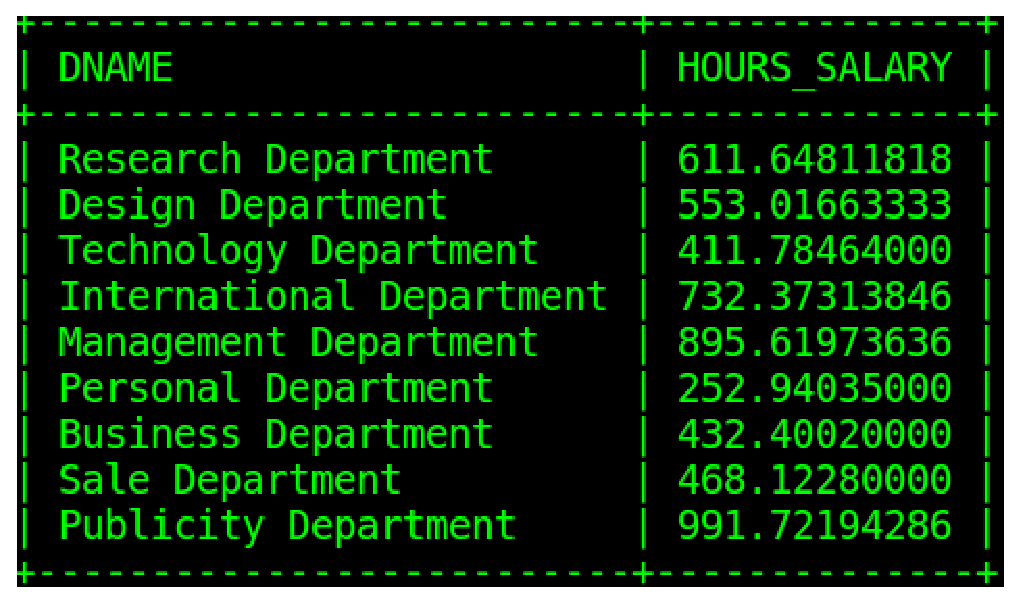
\includegraphics[scale=0.4, bb=0 0 474 274]{media/3.1.9.eps}
        \caption{}\label{fig:9}
    \end{figure}
\end{enumerate}
\subsection{关系数据库COMPANY介绍}
\paragraph{表EMPLOYEE} 其模式如图\ref{fig:emp_pattern}所示,其中\texttt{ESSN}即雇员的身份证号为主键,\texttt{SUPERSSN}即雇员直接上司的身份证号为相对其自身的外键;
对于\texttt{DNO}即雇员所属的部门编号为相对于\texttt{DEPARTMENT}中\texttt{DNO}的外键。
\begin{figure}[htb]
    \centering
    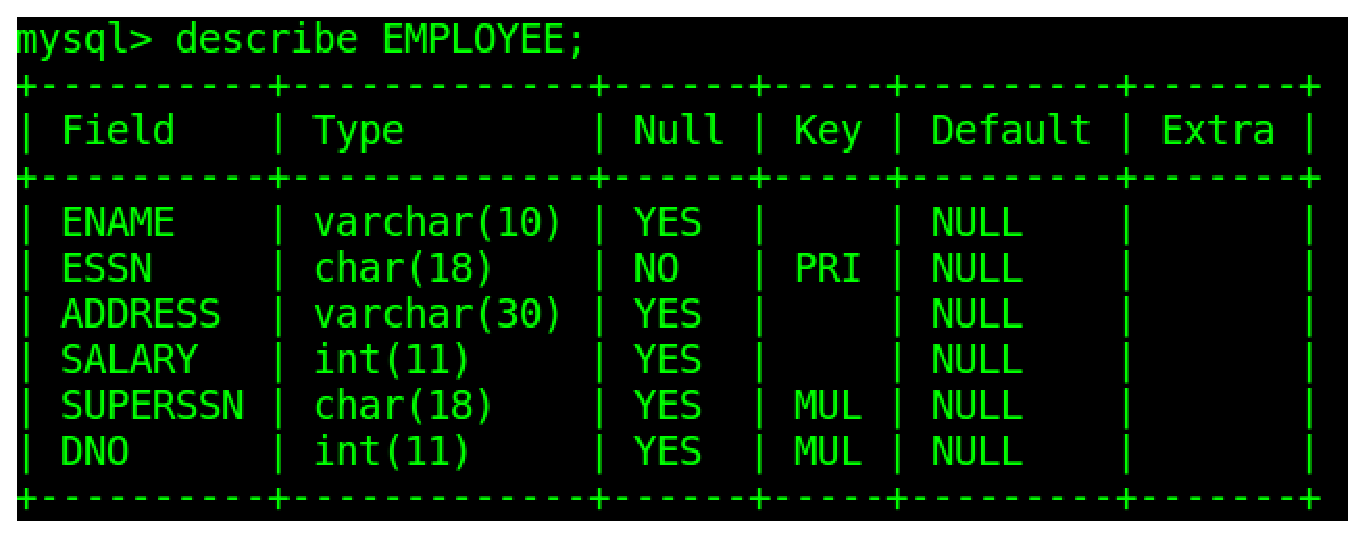
\includegraphics[scale = 0.5, bb=0 0 639 242]{media/employee_pattern.eps}
    \caption{TABLE EMPLOYEE PATTERN}\label{fig:emp_pattern}
\end{figure}
\paragraph{表DEPARTMENT} 其模式如图\ref{fig:dep_pattern}所示,其中\texttt{DNO}即部门编号为主键,\texttt{MGRSSN}即部门领导的身份证号为相对于\texttt{EMPLOYEE}的\texttt{ESSN}的外键。
\begin{figure}[htb]
    \centering
    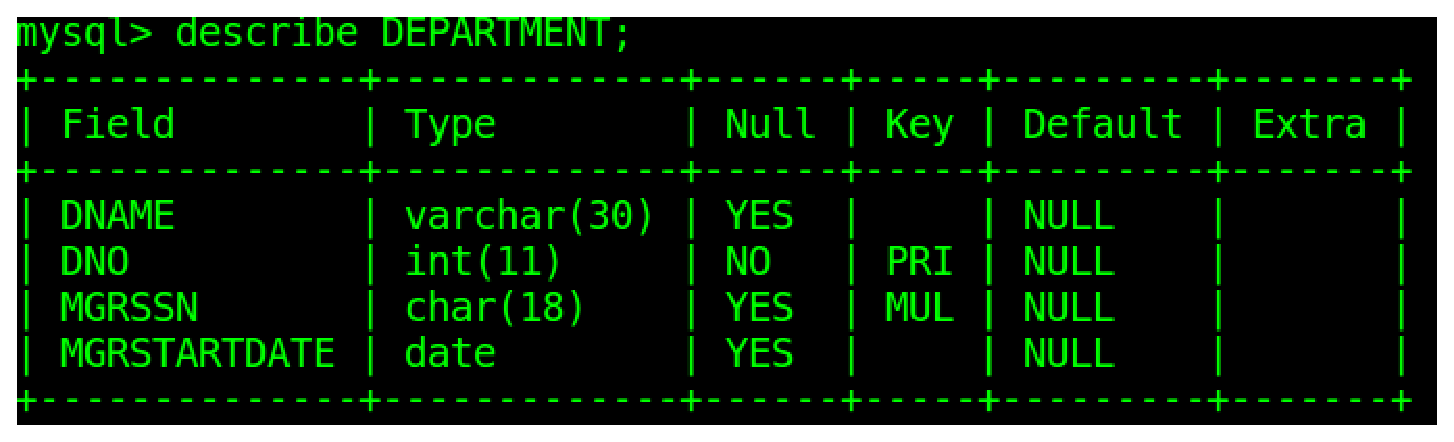
\includegraphics[scale = 0.5, bb=0 0 682 196]{media/department_pattern.eps}
    \caption{TABLE DEPARTMENT PATTERN}\label{fig:dep_pattern}
\end{figure}
\paragraph{表PROJECT} 其模式如图\ref{fig:pro_pattern}所示,其中\texttt{PRO}即工程编号为主键,\texttt{DNO}即所属部门的编号为相对于\texttt{DEPARTMENT}的\texttt{DNO}的外键。
\begin{figure}[htb]
    \centering
    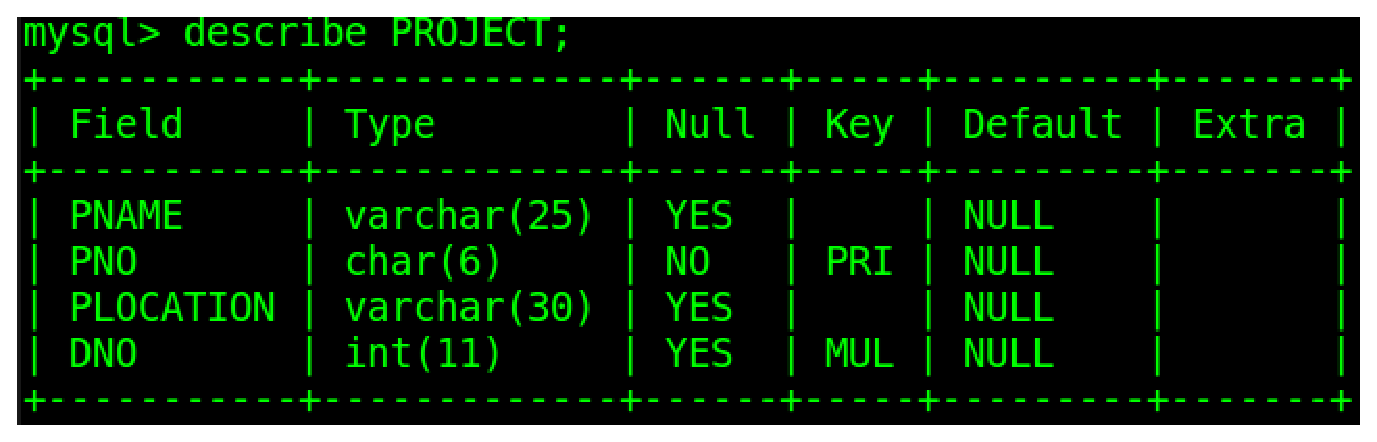
\includegraphics[scale = 0.5, bb=0 0 645 236]{media/project_pattern.eps}
    \caption{TABLE PROJECT PATTERN}\label{fig:pro_pattern}
\end{figure}
\paragraph{表WORKS\_ON} 其模式如图\ref{fig:works_pattern}所示,其中\texttt{ESSN, PNO}为主键。
\begin{figure}[htb]
    \centering
    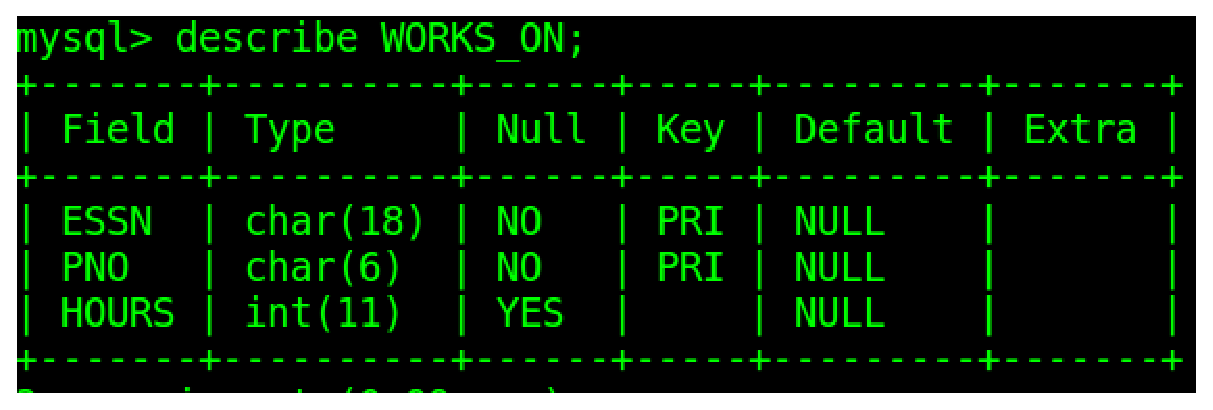
\includegraphics[scale = 0.5, bb=0 0 566 181]{media/works_on_pattern.eps}
    \caption{TABLE WORKS\_ON PATTERN}\label{fig:works_pattern}
\end{figure}
\subsection{数据准备}
\paragraph{表EMPLOYEE} 其共包含89条不同的员工信息,此处仅仅截取了部分信息,如图\ref{fig:employee}所示
\begin{figure}[htb]
    \centering
    \includegraphics[scale = 0.3, bb = 0 0 1487 836]{media/employee.eps}
    \caption{TABLE EMPLOYEE}\label{fig:employee}
\end{figure}
\paragraph{表DEPARTMENT} 其共包含9条不同的部门信息,如图\ref{fig:department}所示。
\begin{figure}[htb]
    \centering
    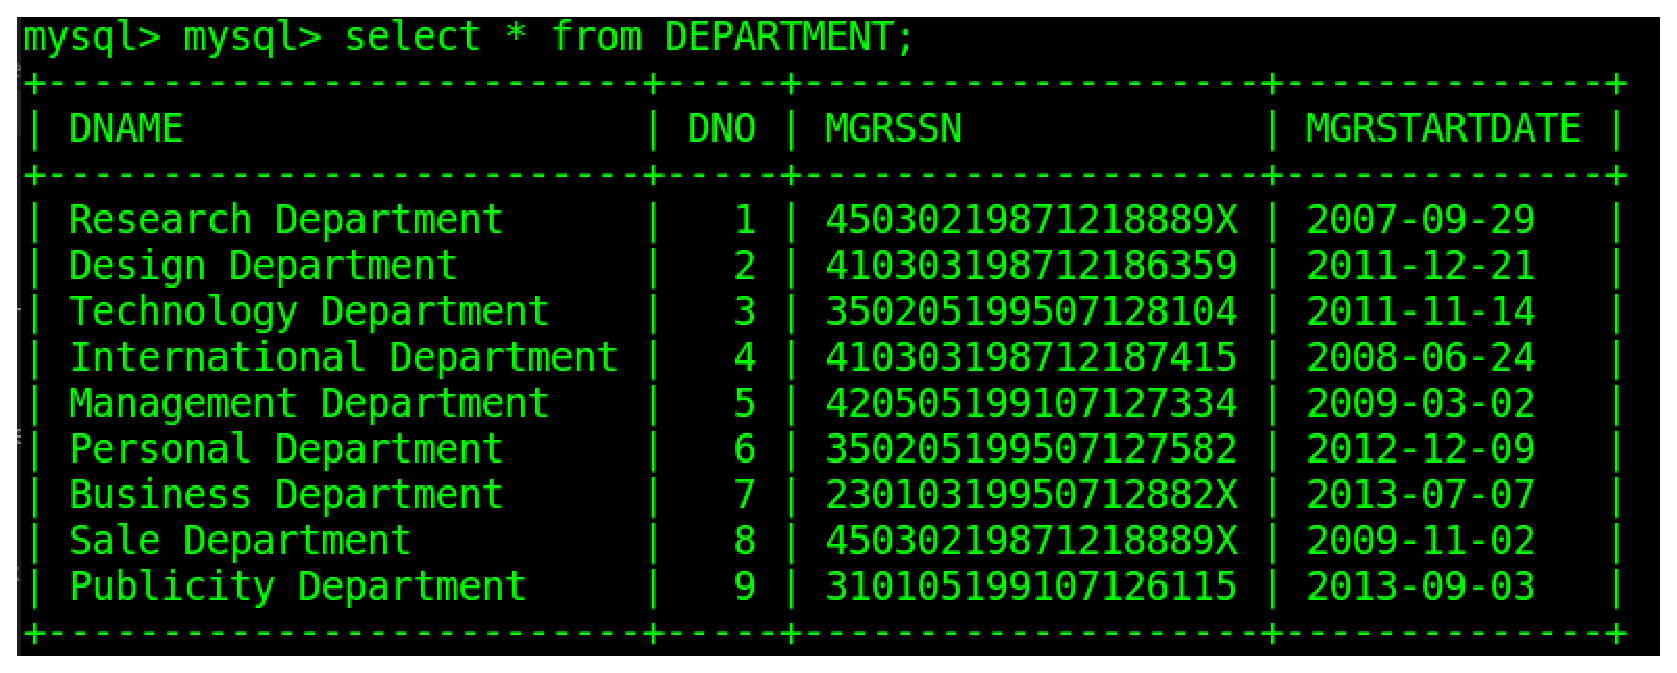
\includegraphics[scale = 0.5, bb = 0 0 789 307]{media/department.eps}
    \caption{TABLE DEPARTMENT}\label{fig:department}
\end{figure}
\paragraph{表PROJECT} 其共包含11条不同的工程信息,如图\ref{fig:project}所示。
\begin{figure}[htb]
    \centering
    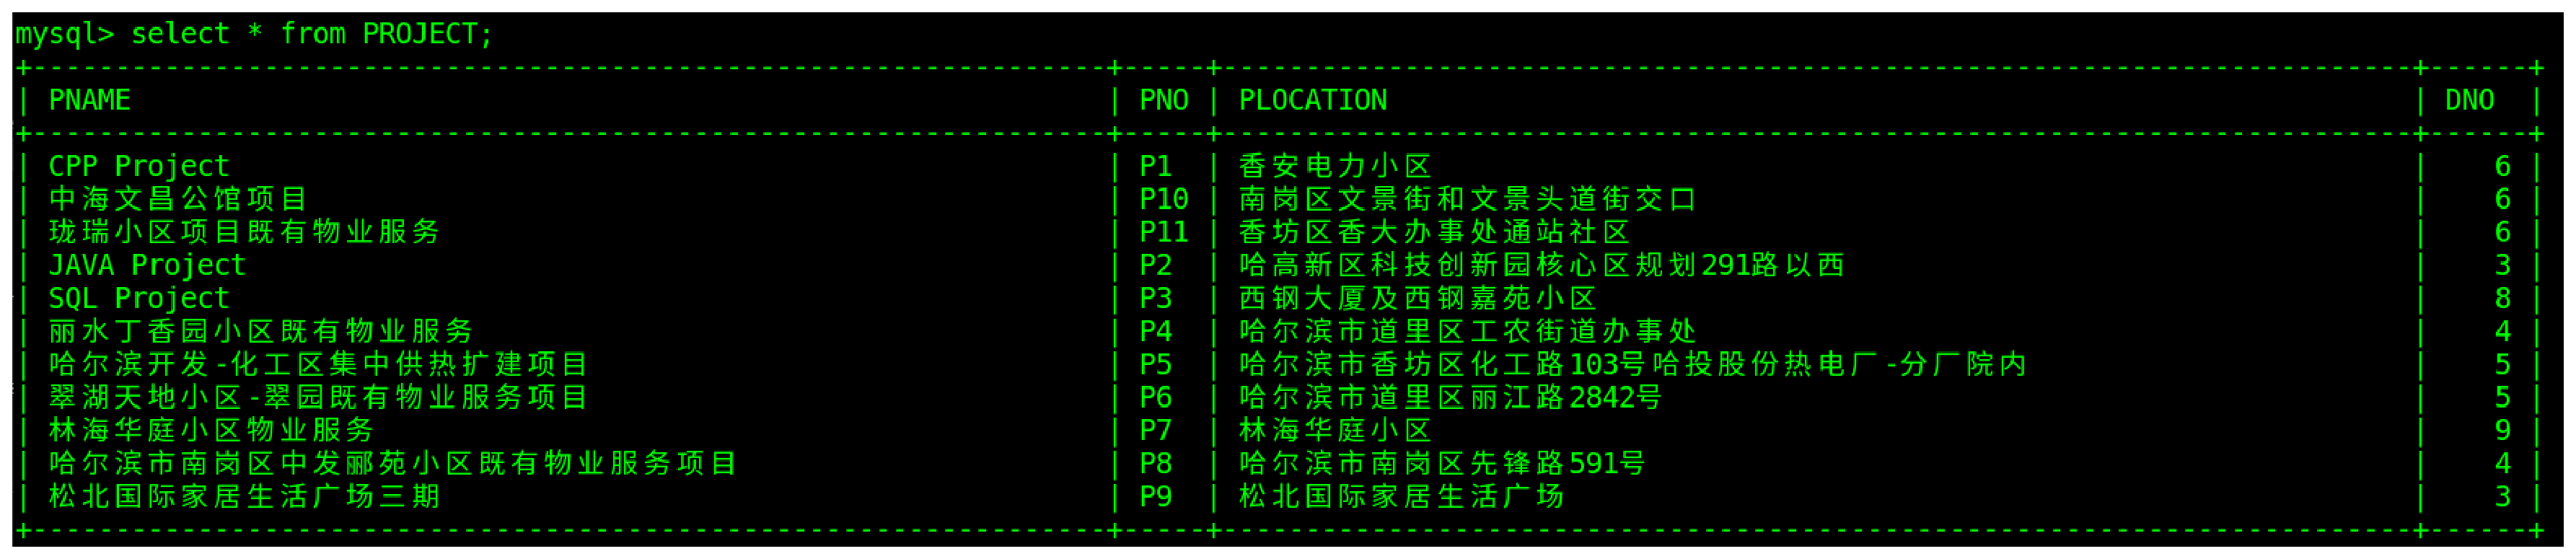
\includegraphics[scale = 0.25, bb = 0 0 1698 356]{media/project.eps}
    \caption{TABLE PROJECT}\label{fig:project}
\end{figure}
\paragraph{表WORKS\_ON} 其共包含了204条不同的工作信息,此处仅仅截取了部分信息,如图\ref{fig:works_on}所示。

\begin{figure}[H]
    \centering
    \includegraphics[scale = 0.5, bb = 0 0 419 375]{media/works_ON.eps}
    \caption{TABLE WORKS\_ON}\label{fig:works_on}
\end{figure}


\section{实验心得}

对于本次实验,准备实验中所需的数据花费了比较多的时间,另外对于如何具体使用MySQL有了比较新的认识,但总体来说实验难度不大。

% \appendix

% \section{源代码}


\end{document}
